\documentclass[times, utf8, diplomski]{fer}
\usepackage{booktabs}
\usepackage{mathtools}
\usepackage{amsmath}
\graphicspath{ {Slike/} }
\begin{document}

% TODO: Navedite broj rada.
\thesisnumber{000}

\title{Polunadzirana klasifikacija rukom pisanih znakova generativnim suparničkim modelima}

\author{Marko Jelavić}

\maketitle

% Ispis stranice s napomenom o umetanju izvornika rada. Uklonite naredbu \izvornik ako želite izbaciti tu stranicu.
\izvornik

\zahvala{Zahvaljujem se mentoru, izv. prof. dr. sc. Siniši Šegviću na podršci i vodstvu kroz diplomski studij te na savjetima i pomoći prilikom izrade diplomskog rada.}

\tableofcontents

\chapter{Uvod}
Klasifikacija rukom pisanih znakova se često koristi kao uvodni problem u područje računalnog vida. Najpoznatiji takav problem je klasifikacija rukom pisanih znamenki (\cite{mnist}) gdje se svakoj slici mora pridijeliti pripadajuća znamenka kao klasa. Pošto se radi o maloj bazi podataka slika niskih rezolucija, rezultati se mogu brzo dobiti te se novi modeli najčešće provjeravaju nad njom. Modeli koji uspješno obavljaju klasifikaciju rukom pisanih znakova najčešće primjenu nalaze kao dio sustava za pretraživanje informacija iz dokumenata. \par

Duboki diskriminativni modeli se smatraju najsuvremenijom tehnologijom iz razloga što pružaju najbolje rezultate u širokom spektru primjena te su najzaslužniji za ekspanziju primjene umjetne inteligencije u industriji. Mana takvih modela je ta što zahtijevaju ogroman broj ručno označenih podataka da bi postigli zadovoljavajuće rezultate. Označavanje podataka je izrazito skup proces te ga se nastoji zaobići. \par

S druge strane, duboki generativni modeli ne zahtijevaju veliku količinu označenih podataka. No, problemi s dosadašnjim modelima se javljaju pri aproksimacijama vjerojatnosnih izračuna pri modeliranju vjerojatnosti ulaznih podataka što usporava proces treniranja modela (\cite{GAN}). U navedenom radu predlaže se model koji se zasniva na suparničkim neuronskim mrežama. 

Model generativnih suparničkih mreža se sastoji od dviju neuronskih mreža, generatorske i diskriminatorske. Spada pod familiju modela bez učitelja, odnosno nisu mu potrebni označeni primjeri za učenje, već samo uči distribuciju ulaznih podataka. Mreža generator ima zadatak naučiti distribuciju ulaznih podataka, a to čini provođenjem latentnih varijabli na ulazu kroz svoje slojeve te kao izlaz daje sliku poput primjera za učenje. Mreža diskriminator ima zadatak odrediti da li je primjer na njenom ulazu generiran ili stvaran. Kroz postupke optimizacije težina, istovremeno se poboljšavaju generator i diskriminator. \par

Nije dugo trebalo da se ovaj model, kao i većina generativnih, pokuša preformulirati u polunadzirani model, te da u konačnici služi kao klasifikator. Pokazalo se da za manji broj ulaznih podataka model funkcionira bolje od izoliranog klasifikatora (\cite{odena}). Upravo to je i cilj ovog rada koji ima zadatak dati uvid u najpoznatije inačice generativnih suparničkih modela, te isprobati model u polunadziranom okruženju na novoj bazi primjera za učenje.

TODO: ŠTO U KOJEM POGLAVLJU

\chapter{Neuronske mreže}
Umjetne neuronske mreže nastale su kao simulacija rada ljudskog mozga. Skupina umjetnih neurona koji su međusobno povezani zajedno čine neuronsku mrežu. Svaki od neurona procesira informaciju na ulazu te daje izlaz. Grupiranje više neurona omogućava modeliranje složenijih relacija koji postoje u podacima na ulazu. Arhitektura neuronske mreže određuje način na koji su umjetni neuroni u istoj spojeni. Također, svaki od neurona može na više načina procesirati ulaze. Neuronske mreže stoga predstavljaju izrazito konfigurabilan model strojnog učenja, koji nalazi široku primjenu u polju umjetne inteligencije.

\section{Umjetni neuron}
Osnovni model umjetnog neurona postavili su autori u radu \cite{mcculloch}. Sastoji se od ulaza u neuron koji su težinski povezani s istim, zatim se otežani ulazi zbrajaju, te se primjenjuje aktivacijska funkcija neurona, kao što je prikazano na slici 2.1. \par

\begin{figure}[!htbp]
    \centering
    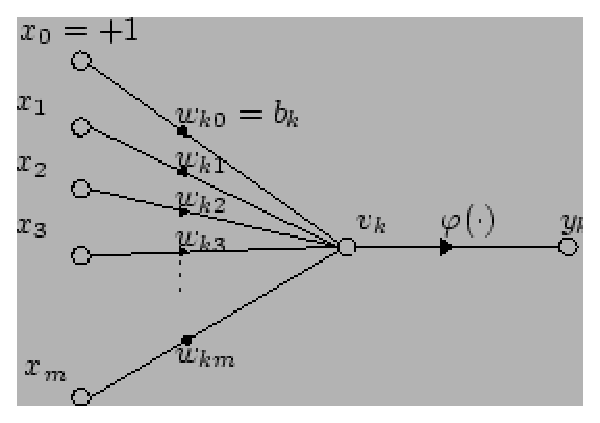
\includegraphics[scale=0.8]{Slike/Artificial_neuron}
    \caption{Umjetni neuron \cite{neuron}}
\end{figure}

Pošto je svim neuronima zajedničko otežano zbrajanje ulaza, svojstva pojedinog neurona zapravo najviše ovise o njegovoj aktivacijskoj funkciji. O njima više u idućoj sekciji.

\subsection{Aktivacijske funkcije}
Aktivacijske funkcije su najznačajnija karakteristika svakog neurona, stoga ne čudi da napredak u razumijevanju pojedinih aktivacijskih funkcija, te predlaganje novih često dovodi do napretka u neuronskim mrežama.

\subsubsection{Prag}
Funkcija praga predložena je u radu \cite{perceptron} gdje je opisan algoritam Perceptrona. Koristi se kao binarni klasifikator. Model Perceptrona je linearan, što znači da algoritam nije u mogućnosti ispravno klasificirati ni najjednostavnije linearno neseparabilne probleme poput prikazanog na slici 2.2. Dokaz za tu tvrdnju daju autori u knjizi \cite{minsky}.

\begin{figure}[!htbp]
    \centering
    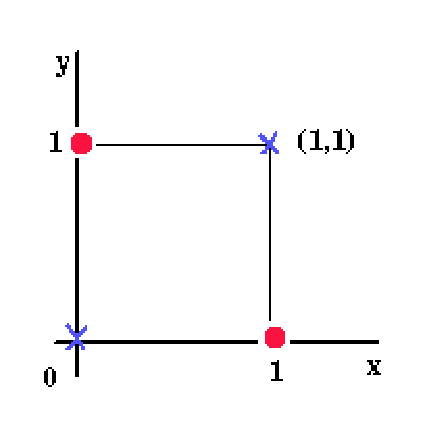
\includegraphics{Slike/xorGraph}
    \caption{XOR problem \cite{xor}}
\end{figure}

Nakon sumiranja otežanih ulaza, funkcija praga se primjenjuje po izrazu 2.1, a graf funkcije je vidljiv na slici 2.3.

\begin{equation}
    f(x)=
    \begin{cases}
      1, & x \geq 0 \\
      0, & x < 0
    \end{cases}
\end{equation}

\pagebreak

\begin{figure}[htbp]
    \centering
    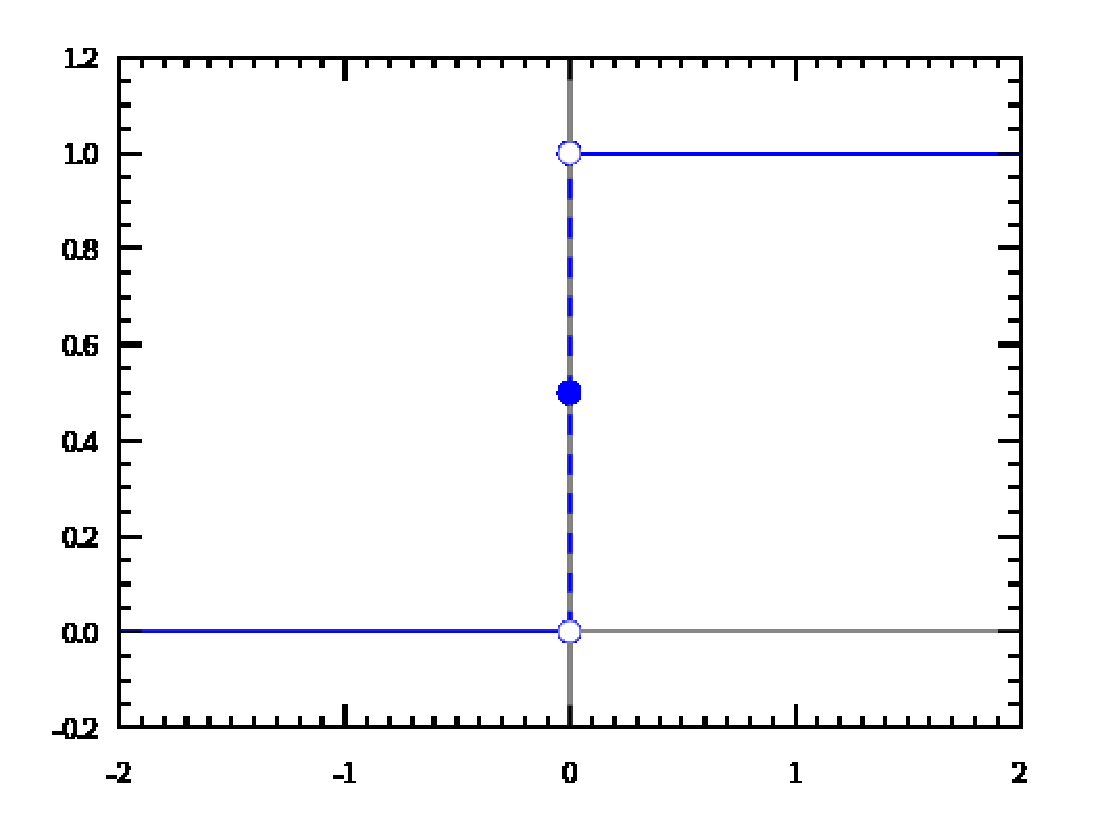
\includegraphics[scale=0.5]{Slike/step}
    \caption{Funkcija praga \cite{step}}
\end{figure}

\subsubsection{Sigmoidalna funkcija}
Sigmoidalna funkcija se prvotno koristila u logističkoj regresiji, te sama logistička regresija može bit interpretirana kao neuron kojem je aktivacijska funkcija sigmoidalna funkcija. Logistička regresija je također linearan klasifikator, no svoju značajnost za razliku od funkcije praga poprima u neuronskim mrežama. \par

Sigmoidalna funkcija je nelinearna aktivacijska funkcija. U neuronskim mrežama izlaz jednog neurona je ulaz drugome. Uvođenjem nelinearnosti preko aktivacijske funkcije omogućava se modeliranje kompleksnijih relacija od linearnih, te širenje primjene modela i na linearno neseparabilne probleme. Zadana je jednadžbom 2.2, a slika 2.4 prikazuje graf funkcije te graf njene derivacije. \par

\begin{equation}
    f(x)=\frac{1}{1 + e^{-x}}
\end{equation}

\begin{figure}[htbp]
    \centering
    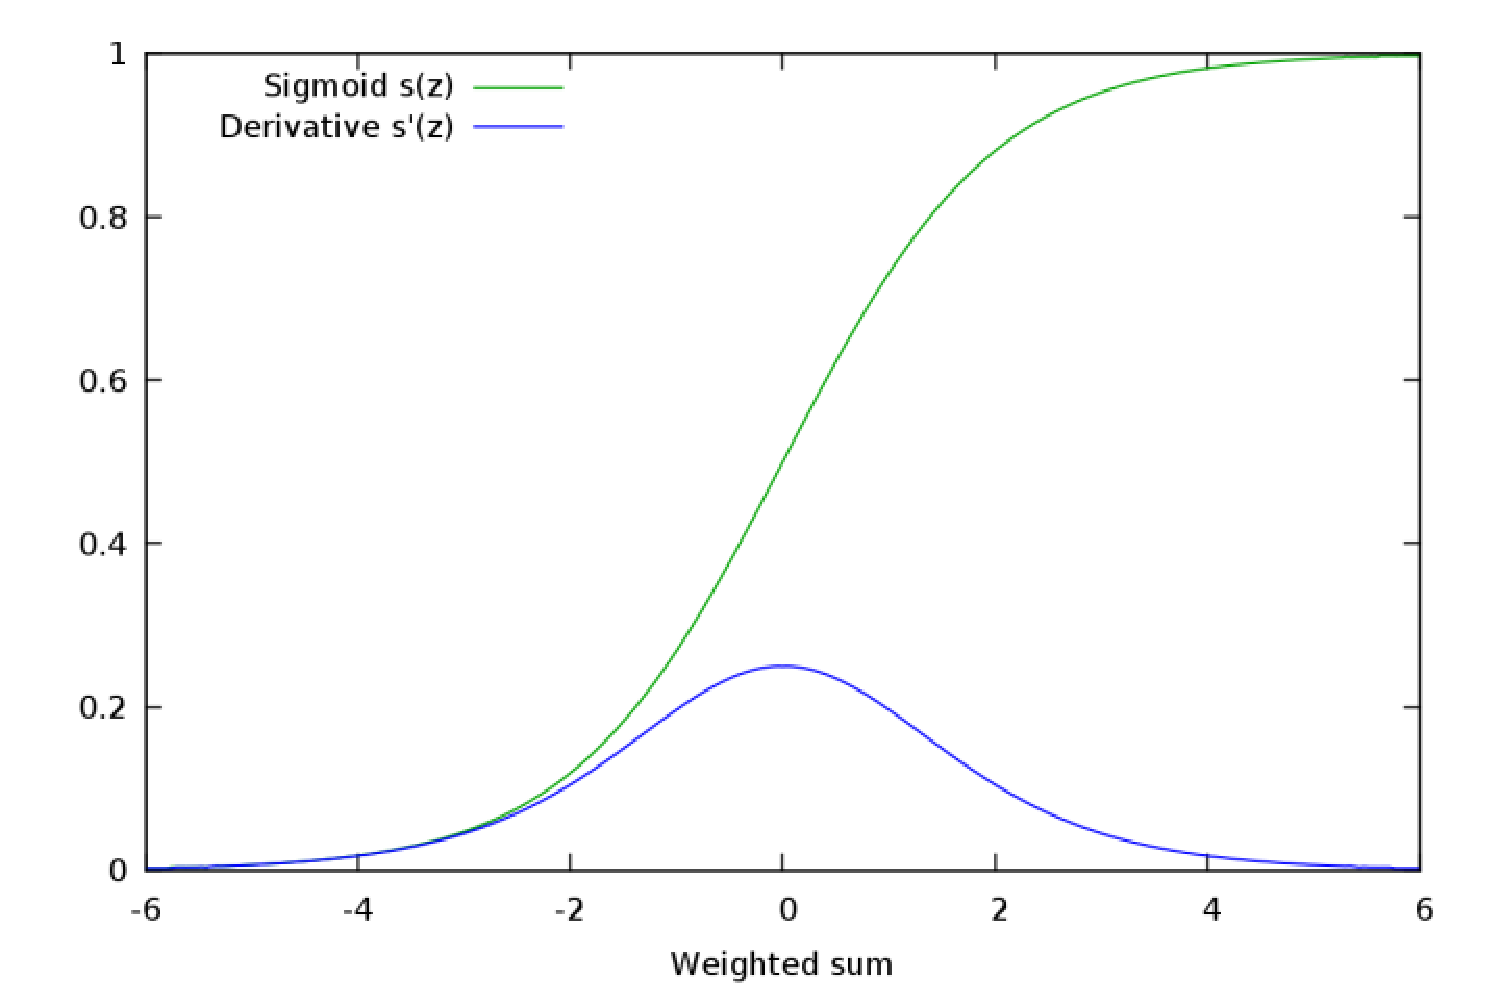
\includegraphics[scale=0.3]{Slike/sigmoid}
    \caption{Sigmoidalna funkcija \cite{sigmoid}}
\end{figure}

Iz grafa funkcije je vidljivo da se sigmoidalnom funkcijom dobije pouzdanost klasifikacije neurona za određeni primjer, što je korisna informacija. No, prva derivacija otkriva manu, a to je problem nestajućeg gradijenta. Ukoliko je izlaz neurona primjerice 0.99, odnosno klasa 1, a zapravo bi trebao biti klasa 0, gradijent je izrazito mali, što znači da će za korekciju klasifikacije trebati velik broj iteracija algoritma gradijentnog spusta.

\subsubsection{Tangens hiperbolni}
Tangens hiperbolni kao aktivacijska funkcija se počeo češće koristiti kao zamjena za sigmoidalnu funkciju iz razloga što ona daje isključivo pozitivne izlaze u intervalu $[0, 1]$ te je centrirana oko $0.5$. To ne predstavlja problem samo jednom neuronu, dok u višeslojnoj neuronskoj mreži koči brzinu konvergencije u postupku učenja. Stoga se predlažu funkcije centrirane oko $0$, a upravo jedna od takvih je tangens hiperbolni \cite{efficient}. Funkcija je zadana jednadžbom 2.3, a graf funkcije i njene derivacije je vidljiv na slici 2.5.

\begin{equation}
    f(x)=tanh(x)=\frac{sinh(x)}{cosh(x)}=\frac{1 - e^{-2x}}{1 + e^{-2x}}
\end{equation}

\begin{figure}[htbp]
    \centering
    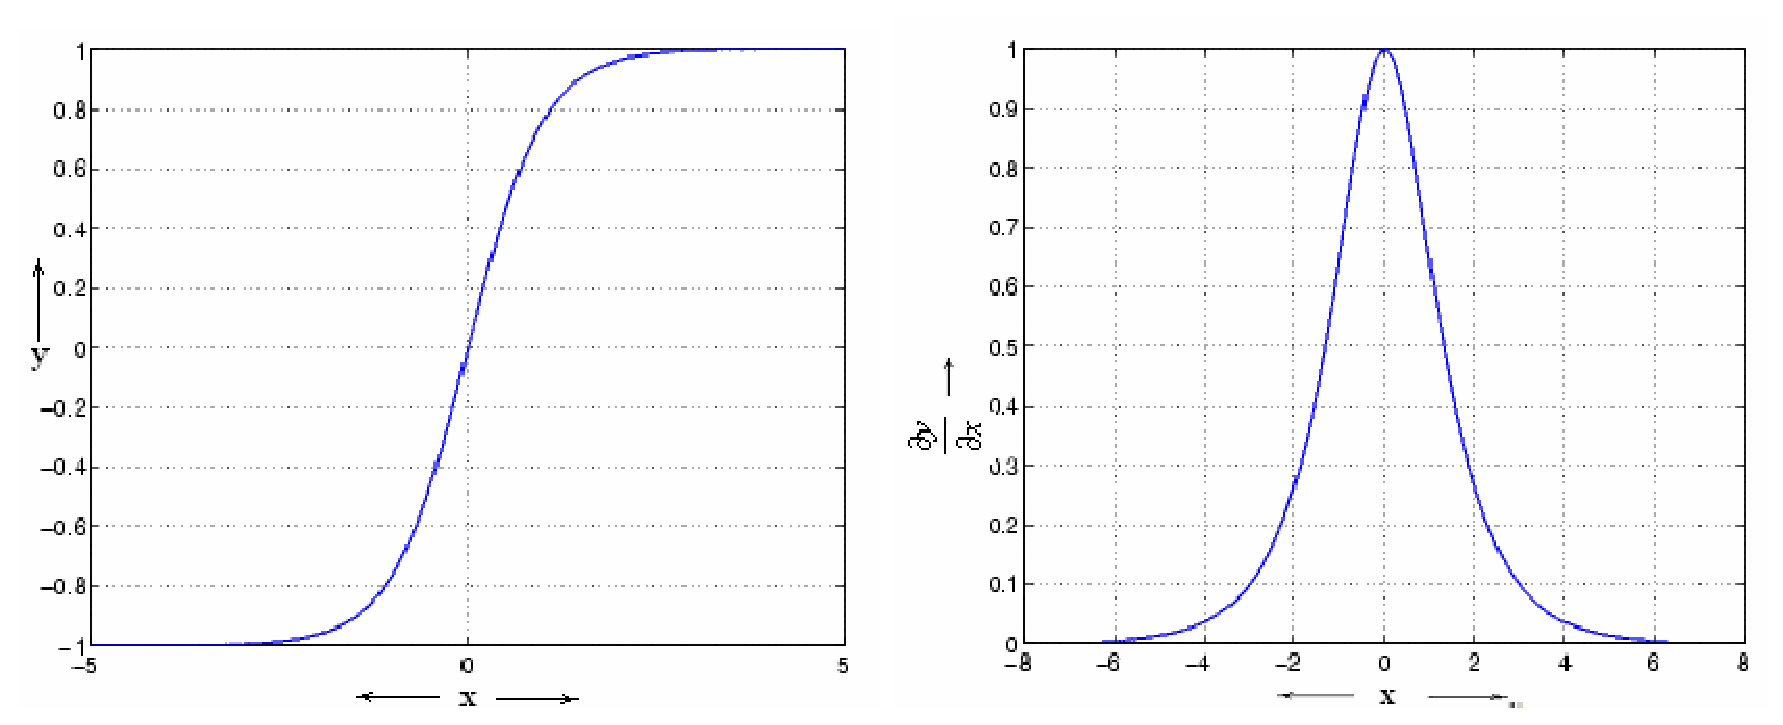
\includegraphics[scale=0.5]{Slike/tanh}
    \caption{Tangens hiperbolni \cite{tanh}}
\end{figure}

Autori u literaturi \cite{efficient} također predlažu modificiranje aktivacijske funkcije u izraz:

\begin{equation}
    f(x)=1.7159 tanh\left( \tfrac{2}{3}x \right).
\end{equation}

Modificirana funkcija za ulaze koji su centrirani na $0$, sa varijancom $1$, daje izlaze koji su također centrirani na $0$ i varijanca bi im trebala biti blizu $1$.

\subsubsection{Rectifier}

U kontekstu neuronskih mreža, rectifier je aktivacijska funkcija čija formula glasi:

\begin{equation}
    f(x)=max(0,x)
\end{equation}

Trenutno je najpopularnija aktivacijska funkcija u arhitekturama dubokih neuronskih mreža (\cite{rect}). Izračunski je vrlo jednostavna, te njen gradijent također ( $0$ za $x<0$, $1$ za $x>0$, nediferencijabilan u $0$), dovodi i do rjeđih aktivacija neurona. Potencijalni problemi su: nije centrirana oko $0$, nediferencijabilna u $0$, neograničena aktivacija te se zna dogodit fenomen umirućih neurona, odnosno neuroni se dovedu u mrtvo stanje iz kojeg ne mogu više izaći, efektivno smanjujući kapacitet neuronske mreže \cite{rect}. Slika 2.6 prikazuje rectifier aktivacijsku funkciju.

\begin{figure}[htbp]
    \centering
    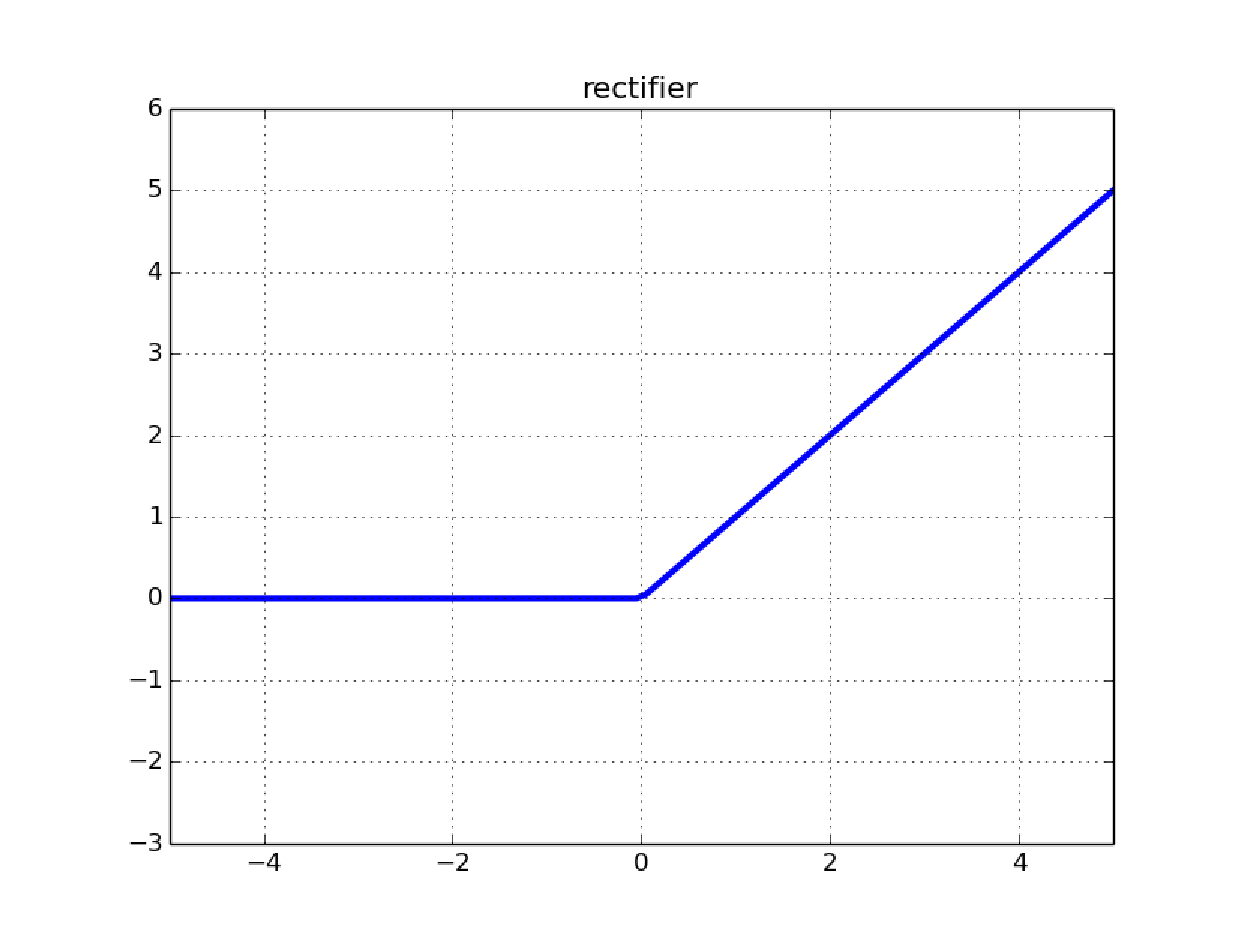
\includegraphics[scale=0.5]{Slike/rect}
    \caption{Rectifier \cite{rectpic}}
\end{figure}

ReLU je lesto korištena skraćenica za rectifier. Poznate varijante su Parametric ReLU (2.6) i ELU (2.7) \cite{rect}.

\begin{equation}
    f(x)=
    \begin{cases}
      x, & x > 0 \\
      ax, & otherwise
    \end{cases}
\end{equation}

\begin{equation}
    f(x)=
    \begin{cases}
      x, & x \geq 0 \\
      a(e^x - 1), & otherwise
    \end{cases}
\end{equation}

\section{Višeslojni perceptron}
Općenita unaprijedna neuronska mreža najčešće se naziva i višeslojnim perceptronom. Sadrži 3 vrste slojeva: ulazni, skriveni i izlazni. Ima 1 ulazni i 1 izlazni sloj, a skrivenih može biti po volji mnogo. Ilustracija jednog višeslojnog perceptrona dana je na slici 2.7.

\begin{figure}[htbp]
    \centering
    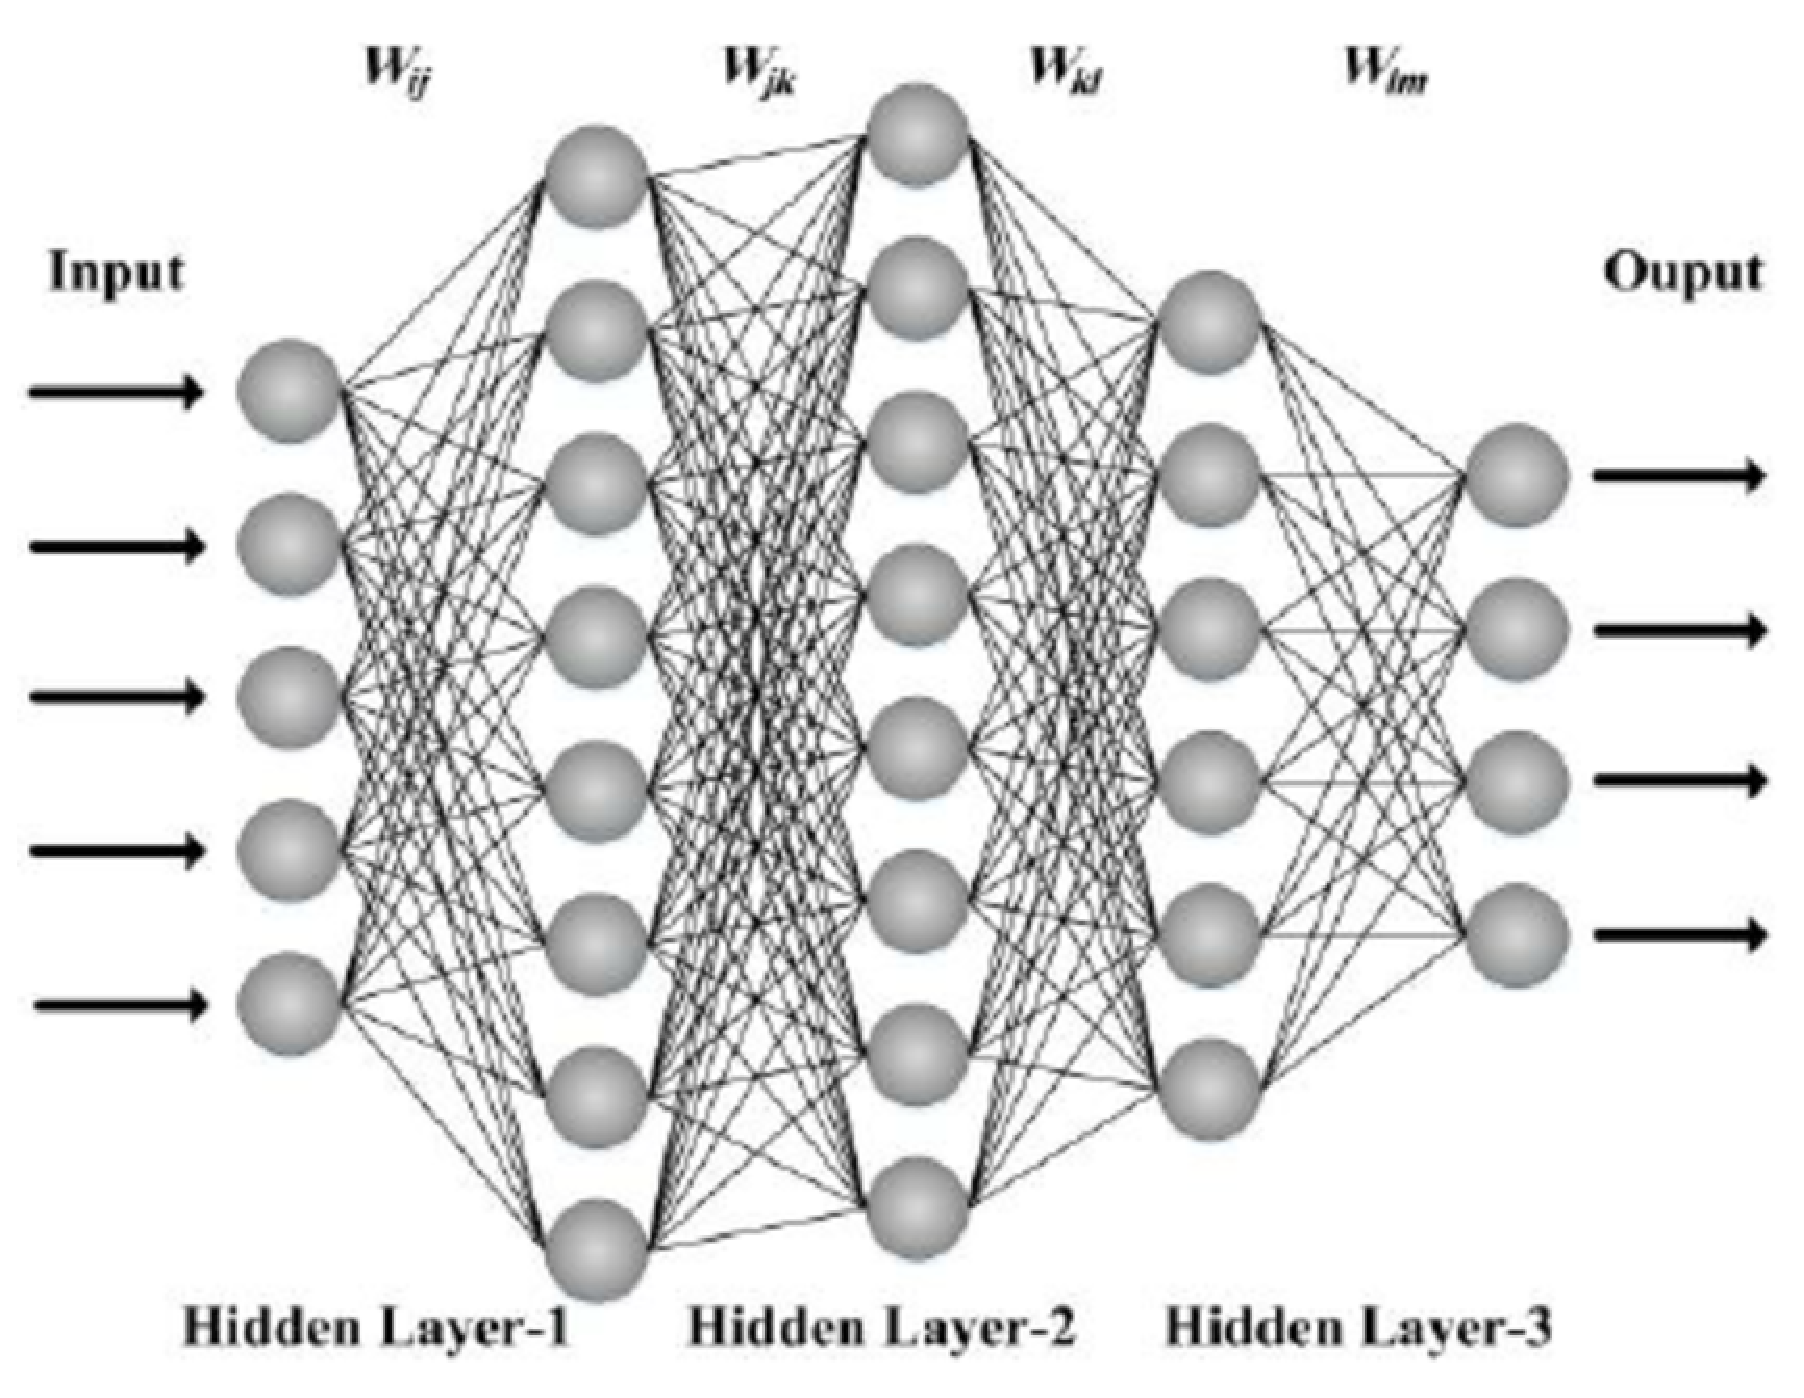
\includegraphics[scale=0.4]{Slike/mlp}
    \caption{Višeslojni perceptron \cite{mlp}}
\end{figure}

Ulazni sloj predstavlja značajke podataka koje obrađujemo, na primjer za sliku, svaki pojedini neuron bi bio jedan piksel slike. U njima se ne vrši nikakva obrada već se samo proslijede prvom idućem skrivenom sloju. Najčešće su slojevi potpuno povezani, odnosno svaki neuron iz prethodnog sloja je povezan sa svakim neuronom u idućem sloju. \par

Skriveni slojevi vrše obradu sumacije otežanih ulaza te primjenu aktivacijske funkcije. Ključ leži u nelinearnosti aktivacijskih funkcija, u protivnom se proizvoljno dubok višeslojni perceptron svodi na najobičniji linearni perceptron. Broj skrivenih slojeva kao i broj neurona u skrivenim slojevima ovisi o problemu koji zadan, no općenito se može reći da neuronska mreža u skrivenim slojevima uči različite reprezentacije ulaznih podataka sa ciljem što uspješnijeg rješavanja problema. Rad \cite{hornik} dokazuje da je neuronska mreža s barem jednim skrivenim slojem služi kao univerzalni funkcijski aproksimator, neovisno o izboru aktivacijske funkcije.\par

Izlazni sloj predstavlja izlaz iz mreže, pri klasifikacijskim problemima to bude vektor pouzdanosti pripadnosti ulaznog primjera određenom broju klasa. Za učenje parametara neuronske mreže koristi se algoritam unazadne propagacije. \par

\subsection{Algoritam unazadne propagacije}
Algoritam unazadne propagacije korigira parametre neuronske mreže s obzirom na gradijent funkcije pogreške. Gradijentni postupci u optimizaciji se koriste već stoljećima, pravilo ulančavanja gradijenata je također otprije poznato stoga je teško navesti sam početak primjene ovog postupka, pa čak i kod neuronskih mreža, no većina se slaže da je metoda popularizirana u radu \cite{backprop}. \par

Algoritam zahtijeva da su aktivacijske funkcije diferencijabilne, te da za zadane ulaze imamo i odgovarajuće izlaze, odnosno primjenjiv je samo u nadziranom učenju. Učenje se odvija u dvije faze:

1) Unaprijedni prolaz odnosno računanje aktivacija neurona za zadani ulaz sve do izlaza mreže, te posljedično računanje izlaza mreže za zadani ulaz.

2) Unazadni prolaz gdje se računa odstupanje izlaza mreže od traženog izlaza zadanog primjera, propagira se unazad kroz mrežu računajući grešku pri svakom od neurona, te naposlijetku se obavlja korekcija težina mreže jednom od gradijentnih metoda.

Ulančavanje gradijenata pokazat ćemo na jednostavnom primjeru mreže sa ulaznim, jednim skrivenim, te izlaznim slojem. Neka je zadano N primjera za učenje oblika $(x\textsubscript{n},y\textsubscript{n})$. Neka mreža koristi sigmoidalnu aktivacijsku funkciju u skrivenom i izlaznom sloju, te minimizira funkciju srednje kvadratne pogreške

\begin{equation}
	E=\frac{1}{2N}\sum_{n=1}^{N}(y\textsubscript{n} - o\textsubscript{n})^2
\end{equation}

gdje je $o\textsubscript{n}$ izlaz mreže za ulaz $x\textsubscript{n}$. Za početak ćemo pokazati izraz za podešavanje parametara izlaznog sloja. Neka \textbf{W\textsuperscript{(i)}} označava matricu parametara izlaznog sloja, a \textbf{h\textsubscript{n}} vektor izlaza srednjeg sloja za n-ti primjer, odnosno ulaza u izlazni sloj, kojemu je dodan član pristranosti $1$. Tada derivacija funkcije greške po parametrima izlaznog sloja izgleda:

\begin{equation}
	\frac{\partial E}{\partial \textbf{W\textsuperscript{(i)}}} = \frac{\partial E}{\partial o\textsubscript{n}} \frac{\partial o\textsubscript{n}}{\partial net\textsubscript{n}\textsuperscript{(i)}} \frac{\partial net\textsubscript{n}\textsuperscript{(i)}}{\partial \textbf{W\textsuperscript{(i)}}}
\end{equation}

\begin{equation}
	\frac{\partial E}{\partial o\textsubscript{n}} = -\frac{1}{N}\sum_{n=1}^{N}(y\textsubscript{n} - o\textsubscript{n})
\end{equation}

Pošto je $o\textsubscript{n}$ sigmoidalna funkcija, njena derivacija iznosi:

\begin{equation}
	\frac{\partial o\textsubscript{n}}{\partial net\textsubscript{n}\textsuperscript{(i)}} = o\textsubscript{n} (1 - o\textsubscript{n})	
\end{equation}
$net$ označava ulazni sloj (u ovom slučaju skriveni sloj) pomnožen s matricom težina odnosno parametara, u ovom slučaju izlaznog sloja:
\begin{equation}
	net\textsubscript{n}\textsuperscript{(i)} = \textbf{W\textsuperscript{(i)}} h\textsubscript{n}
\end{equation}
\begin{equation}
	\frac{\partial net\textsubscript{n}\textsuperscript{(i)}}{\partial \textbf{W\textsuperscript{(i)}}} = h\textsubscript{n}
\end{equation}

Izračunavši sve potrebne parcijalne derivacije konačan izraz za gradijent izlaznog sloja glasi:

\begin{equation}
	\frac{\partial E}{\partial \textbf{W\textsuperscript{(i)}}} = -\frac{1}{N}\sum_{n=1}^{N}(y\textsubscript{n} - o\textsubscript{n})o\textsubscript{n} (1 - o\textsubscript{n})h\textsubscript{n}
\end{equation}
Često se koristi i skraćena verzija zapisa:
\begin{equation}
	\frac{\partial E}{\partial \textbf{W\textsuperscript{(i)}}} = -\frac{1}{N}\sum_{n=1}^{N} \delta\textsubscript{n}\textsuperscript{(i)}h\textsubscript{n}
\end{equation}
gdje je
\begin{equation}
	\delta\textsubscript{n}\textsuperscript{(i)} = (y\textsubscript{n} - o\textsubscript{n})o\textsubscript{n} (1 - o\textsubscript{n})
\end{equation}
Neka $\textbf{W\textsuperscript{(h)}}$ predstavlja matricu parametara skrivenog sloja, a neka $x\textsubscript{n}$ predstavlja ulazni vektor u skriveni sloj, također proširen s članom pristranosti $1$. Da bi dobili gradijent skrivenog sloja moramo se vratit korak unatrag:

\begin{equation}
	\frac{\partial net\textsubscript{n}\textsuperscript{(i)}}{\partial \textbf{W\textsuperscript{(h)}}} = \textbf{W\textsuperscript{(i)}} \frac{\partial h\textsubscript{n}}{\partial \textbf{W\textsuperscript{(h)}}} 
\end{equation}
Odnosno nastavljamo s parcijalnim deriviranjem unatrag kroz mrežu. Trenutno gradijent izgleda:

\begin{equation}
	\frac{\partial E}{\partial \textbf{W\textsuperscript{(i)}}} = -\frac{1}{N}\sum_{n=1}^{N} \delta\textsubscript{n}\textsuperscript{(i)}\textbf{W\textsuperscript{(i)}}\frac{\partial h\textsubscript{n}}{\partial \textbf{W\textsuperscript{(h)}}}
\end{equation}
\begin{equation}
\frac{\partial h\textsubscript{n}}{\partial \textbf{W\textsuperscript{(h)}}} = \frac{\partial h\textsubscript{n}}{\partial net\textsubscript{n}\textsuperscript{(h)}}\frac{\partial net\textsubscript{n}\textsuperscript{(h)}}{\partial \textbf{W\textsuperscript{(h)}}}
\end{equation}
Pošto je $h\textsubscript{n}$ izlaz sigmoidalne aktivacijske funkcija, derivacija glasi:
\begin{equation}
\frac{\partial h\textsubscript{n}}{\partial net\textsubscript{n}\textsuperscript{(h)}} = h\textsubscript{n}(1 - h\textsubscript{n})
\end{equation}
\begin{equation}
net\textsubscript{n}\textsuperscript{(h)} = \textbf{W\textsuperscript{(h)}}x\textsubscript{n}
\end{equation}
\begin{equation}
\frac{\partial net\textsubscript{n}\textsuperscript{(h)}}{\textbf{W\textsuperscript{(h)}}} = x\textsubscript{n}
\end{equation}
Izračunom svih potrebnih parcijalnih derivacija dobije se:
\begin{equation}
\frac{\partial h\textsubscript{n}}{\partial \textbf{W\textsuperscript{(h)}}} = h\textsubscript{n}(1 - h\textsubscript{n})x\textsubscript{n}
\end{equation}
Konačan gradijent parametara skrivenog sloja glasi:
\begin{equation}
	\frac{\partial E}{\partial \textbf{W\textsuperscript{(h)}}} = -\frac{1}{N}\sum_{n=1}^{N} \delta\textsubscript{n}\textsuperscript{(i)}\textbf{W\textsuperscript{(i)}}h\textsubscript{n}(1 - h\textsubscript{n})x\textsubscript{n}
\end{equation}
ili skraćeno:
\begin{equation}
	\frac{\partial E}{\partial \textbf{W\textsuperscript{(h)}}} = -\frac{1}{N}\sum_{n=1}^{N} \delta\textsubscript{n}\textsuperscript{(h)}x\textsubscript{n}
\end{equation}
gdje je 
\begin{equation}
\delta\textsubscript{n}\textsuperscript{(h)} = \delta\textsubscript{n}\textsuperscript{(i)}\textbf{W\textsuperscript{(i)}}h\textsubscript{n}(1 - h\textsubscript{n})
\end{equation}
Ulančavanje se nastavlja po istom principu i za više slojeva. Učenje se vrši optimizacijskim postupcima koji se temelje na gradijentima. Nakon što smo pokazali kako se računaju gradijenti s obzirom na funkciju pogreške neuronske mreže, slijedi pregled odabranih optimizacijskih metoda.

\subsubsection{Gradijentni spust}
Gradijentni spust je osnovna numerička metoda minimizacije funkcije pogreške u strojnom učenju. Promatramo funkciju pogreške kao funkciju parametara algoritma, te optimiziramo parametre algoritma u smjeru minimalne greške te funkcije. Gornji primjer pokazuje kako izračunati gradijente parametara, dok se podešavanje parametara odvija po idućoj formuli:

\begin{equation}
\textbf{W\textsuperscript{(n+1)}} = \textbf{W\textsuperscript{(n)}} - \eta\frac{\partial E}{\partial \textbf{W\textsuperscript{(n)}}}
\end{equation}

gdje je $n+1$ vremenska oznaka buduće vrijednosti, $n$ trenutne, a $\eta$ nazivamo stopom učenja, ona određuje koliki će biti pomak u smjeru gradijenta. Kao i svi numerički postupci, stabilnost ovog postupka ovisi o  odabiru vrijednosti $\eta$. \par

Postoje tri različita načina osvježavanja parametara. Stohastički gradijentni spust se temelji na tome da se za svaki primjer izračunaju gradijenti i odma osvježe parametri modela. Grupni gradijentni spust zbroji gradijente svih primjera, uzme prosjek tako da zbroj podijeli s brojem primjera te onda osvježi parametre modela. Treći način je kompromisni, ujedno i najkorišteniji, u kojem se odredi nekakav $n$ koji je veličina grupe nakon koje će model osvježavati parametre. Stohastički gradijentni spust je vremenski skup radi čestog osvježavanja parametara, no otporniji je na lokalne optimume. Grupni gradijentni spust radi izrazito dobro pri konveksnim problemima, no ne i u onim gdje krivulje funkcije pogreške imaju mnogo lokalnih optimuma. Također je memorijski zahtjevno koristiti sve primjere za učenje odjednom. Upravo zato je i najkorišteniji kompromisni način, jer veličinom grupe kontroliramo prednosti i mane oba načina. Postupak optimizacije se vrši do zadovoljavanja zadanih kriterija konvergencije ili do isteka postavljenog maksimalnog broja iteracija.\par

\subsubsection{Momentum}
Momentum metoda osim gradijenta uzima u obzir i gradijent u prethodnom koraku. Cilj je dobiti konzistentniji smjer gradijenta, dajući mu "širu sliku" kretnje po hiperravnini funkcije pogreške, a ne samo trenutno stanje. Predložena je kao poboljšanje nad stohastičkim gradijentnim spustom u radu \cite{backprop}.

\begin{equation}
\Delta W\textsuperscript{(n)} = \eta\frac{\partial E}{\partial \textbf{W\textsuperscript{(n)}}} + \alpha \Delta W\textsuperscript{(n-1)}
\end{equation}
\begin{equation}
W\textsuperscript{(n+1)} = W\textsuperscript{(n)} - \Delta W\textsuperscript{(n)}
\end{equation}

\subsubsection{RMSProp}
RMSProp (engl. \textit{Root Mean Square Propagation}) je varijanta gradijentnog spusta s dodanim parametrom. Uz stopu učenja $\eta$, postoji i stopa zaboravljanja $\gamma$. Osnovna ideja je da model na početku brzo podešava težine, no što je bliži konvergenciji gradijenti su manji stoga je i proces učenja sporiji. RMSProp to mijenja tako što modificira stopu učenja obrnuto proporcionalno magnitudi gradijenta. Optimizacijski postupak je predložen u literaturi \cite{rmsprop}.

\begin{equation}
v\textsuperscript{(n)} = \gamma v\textsuperscript{(n-1)} + (1-\gamma)\left(\frac{\partial E}{\partial \textbf{W\textsuperscript{(n)}}}\right)^2
\end{equation}

Po izrazu 2.28 modificiramo stopu učenja. $v\textsuperscript{(n)}$ označava magnitudu gradijenta u $n$-tom koraku, a pri tom koristi i magnitudu gradijenta u $n-1$ koraku, sve zajedno parametrizirano s $\gamma$. Sada postupak osvježavanja parametara izgleda:

\begin{equation}
\textbf{W\textsuperscript{(n+1)}} = \textbf{W\textsuperscript{(n)}} - \frac{\eta}{\sqrt{v\textsuperscript{(n)}}}\frac{\partial E}{\partial \textbf{W\textsuperscript{(n)}}}
\end{equation}

\subsubsection{Adam}
Adam (engl. \textit{Adaptive Moment Estimation}) je kombinacija Momentum i RMSProp metoda. Postupak je prezentiran u radu \cite{adam}, gdje autori detaljnije izvode izraza u algoritmu, pružaju eksperimentalne rezultate kao dokaz te predlažu odabir parametara za koje smatraju da su robusni i široko primjenjivi.

\begin{equation}
m\textsubscript{w}\textsuperscript{(n+1)} = \beta\textsubscript{1}m\textsubscript{w}\textsuperscript{(n)} + (1 - \beta\textsubscript{1})\frac{\partial E}{\partial \textbf{W\textsuperscript{(n)}}}
\end{equation}

\begin{equation}
v\textsubscript{w}\textsuperscript{(n+1)} = \beta\textsubscript{2}v\textsubscript{w}\textsuperscript{(n)} + (1 - \beta\textsubscript{2})\left(\frac{\partial E}{\partial \textbf{W\textsuperscript{(n)}}}\right)^2
\end{equation}

\begin{equation}
\hat{m}\textsubscript{w}\textsuperscript{(n)} = \frac{m\textsubscript{w}\textsuperscript{(n)}}{1 - \beta_{1}^n}
\end{equation}

\begin{equation}
\hat{v}\textsubscript{w}\textsuperscript{(n)} = \frac{v\textsubscript{w}\textsuperscript{(n)}}{1 - \beta_{2}^n}
\end{equation}

\begin{equation}
\textbf{W\textsuperscript{(n+1)}} = \textbf{W\textsuperscript{(n)}} - \eta\frac{\hat{m}\textsubscript{w}\textsuperscript{(n)}}{\sqrt{\hat{v}\textsuperscript{(n)}} + \epsilon}
\end{equation}

Iz gornjih relacija očigledno je da postupak ima 4 parametra. Parametri $\beta_1$ i $\beta_2$ su faktori zaboravljanja za prvi, odnosno drugi moment gradijenata, $\epsilon$ je mali korekcijski faktor za slučaj izbjegavanja dijeljenja s $0$ i $\eta$ koja je stopa učenja kao i u prethodnim gradijentnim postupcima. Relacije 2.32 i 2.33 daju pristrane procjenitelje prvog i drugog momenta gradijenta stoga se korigiraju za faktor pristranosti, pa se dobiju nepristrani procjenitelji iz relacija 2.34 i 2.35.

\pagebreak

\section{Konvolucijske neuronske mreže}
Konvolucijske neuronske mreže, za razliku od višeslojnih perceptrona, koriste konvolucijske slojeve o kojima će biti govora kasnije u ovoj sekciji. Prva takva zabilježena mreža nalazi se u literaturi \cite{neocognitron}, no za popularizaciju istih uglavnom se navodi rad \cite{convnet}. Najveći napredak su postigle u polju računalnog vida, gdje su pri nekim problemima postigle i nadljudske rezultate. 

\subsection{Konvolucija}
U obradi slike koristimo 2D konvolucijski operator nad diskretnim vrijednostima. Stoga operator 2D diskretne konvolucije se definira preko idućeg izraza:

\begin{equation}
f(x,y) * g(x,y) = \sum_{n_1 = -\infty}^\infty \sum_{n_2 = -\infty}^\infty f(n_1, n_2) g(x - n_1, y - n_2)
\end{equation}

Na prvi pogled jednostavan izraz, oko kojeg je teško razviti intuiciju \cite{convolution}. No, gornji izraz je općenit slučaj za konvoluciju dva dvodimenzionalna signala, na primjerima ćemo vidjeti da se u obradi slike radi o mnogo jednostavnijem slučaju. Slika 2.8 prikazuje 2 često korištena Laplace filtra.\par

\begin{figure}[htbp]
    \centering
    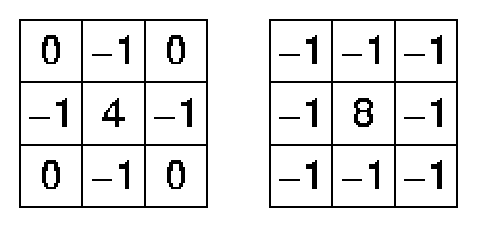
\includegraphics[scale=1]{Slike/laplace}
    \caption{Laplace filter \cite{laplace}}
\end{figure}

\begin{figure}[htbp]
    \centering
    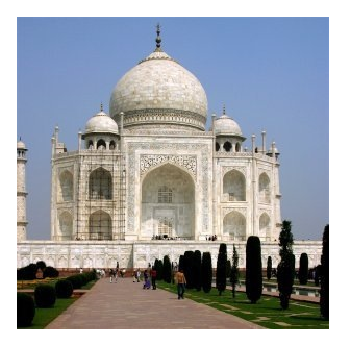
\includegraphics[scale=0.75]{Slike/taj_orig}
    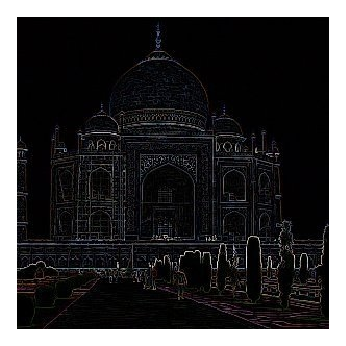
\includegraphics[scale=0.75]{Slike/edge-taj-laplace}
    \caption{Primjer djelovanja Laplace filtra na sliku \cite{laplaceexample}}
\end{figure}

\pagebreak

Konvolucijskim prozorom se prolazi kroz cijelu sliku, sumirajući težinski pikselne vrijednosti, te na izlazu dobijemo obrađenu sliku. Primjer djelovanja Laplace filtra dan je na slici 2.9.\par

Upravo ideja da se koriste konvolucijski operatori s filtrima koji su naučeni, a ne predodređeni, omogućile su neuronskim mrežama izrazit uspjeh u polju računalnog vida. Pri obradi slike to je od iznimne važnosti jer se postiže lokalna osjetljivost i dijeljenje parametara, odnosno model sam nauči mapiranje iz slike u prostor značajki koji je kasnije povezan na potpuno povezani sloj najčešće, ili nekakav drugi klasifikator. \par

Korištenje konvolucijskih slojeva omogućava slojevitiju mrežu, pošto su parametri dijeljeni, problem naglog rasta broja parametara sa slojevitošću je manji nego kod potpuno povezanih slojeva višeslojnog perceptrona. Stoga se konvolucijski slojevi bliže ulaznoj slici najčešće fokusiraju na detekciju značajki niske razine poput rubova i linija, dok kasniji konvolucijski slojevi modeliraju značajke viših razina poput razumijevanja scene i objekata.

\subsection{Slojevi sažimanja}
Uz konvolucijske slojeve često se u arhitekturama konvolucijskih neuronskih mreža mogu pronaći i slojevi sažimanja. Najčešće korišten operator je sažimanje po maksimalnom odzivu, no postoji sažimanje po minimalnom i prosječnom odzivu. Slojevi sažimanja općenito primaju sliku te zatim po regjiama slike primjenjuju odabrani operator. Postižu smanjenje dimenzionalnosti, posljedično i smanjenje broja parametara modela što spriječava prenaučenost.

\begin{figure}[htbp]
    \centering
    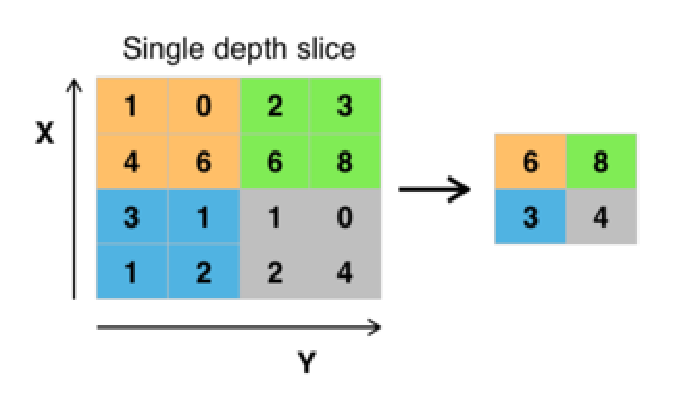
\includegraphics[scale=1]{Slike/Max_pooling}
    \caption{Primjer sažimanja po maksimalnom odzivu \cite{maxpoolexample}}
\end{figure}

\subsection{Arhitektura konvolucijskih neuronskih mreža}
Konvolucijske neuronske mreže primaju 2D ulaze poput slike, provlače ih kroz prvi konvolucijski sloj, nakon što se dobije prva mapa značajki, neuroni konvolucijskog sloja primjenjuju aktivacijske funkcije te se nakon toga vrši sloj sažimanja. Taj proces se ponavlja ovisno o tome koliko arhitektura mreže ima konvolucijskih slojeva. Izlaz zadnjeg konvolucijskog sloja je također mapa značajki koja se zatim "izravna" te se predaje potpuno povezanim slojevima. \par

\begin{figure}[htbp]
    \centering
    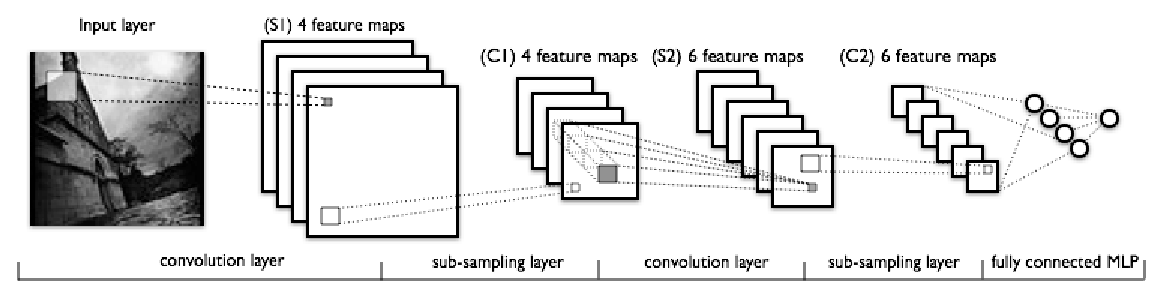
\includegraphics[scale=0.75]{Slike/mylenet}
    \caption{Primjer arhitekture konvolucijske neuronske mreže \cite{mylenet}}
\end{figure}

Autori u radu \cite{striving} predlažu pojednostavljenja u arhitekturama konvolucijskih mreža. Predlažu izbacivanje slojeva sažimanja te nadomještajući to proširenjem koraka konvolucijskih filtara. \par

U zadnje vrijeme počeo se koristi pojam prijenosa učenja (engl. \textit{transfer learning}). Odnosi se na to da se mreža naučena nad jednim skupom podataka primjenjuje i nad drugim skupovima podataka. Često samo zahtijeva modifikacije nad posljednjim klasifikacijskim slojem jer se skupovi podataka razlikuju u broju klasa. Proces treniranja je isti, no praksa je pokazala da značajke naučene na skupom A služe bolje od učenja nove mreže s incijaliziranim težinama. Stoga nije ni čudo da dosada već postoji par standardnih, pretreniranih arhitektura koje se dalje prilagođavaju nad ostalim skupovima podataka.

\pagebreak

\section{Grupna normalizacija}
Grupna (engl. \textit{batch}) normalizacija je metoda predstavljena u literaturi \cite{batchnorm}. Motivacija je parametrizirano normalizirati ulaze u svaki sloj neuronske mreže pošto se distribucije ulaza u slojeve mijenjaju kroz treniranje. Gore navedeni problem povlači i druge probleme poput opreznog postavljanja stope učenja te inicijalizacije parametara mreže. Grupna normalizacija do neke mjere eliminira te probleme. Grupe se normaliziraju po sljedećim izrazima:

\begin{equation}
\mu_B = \frac{1}{m}\sum_{i=1}^m x_i
\end{equation}

\begin{equation}
\sigma_B^2 = \frac{1}{m}\sum_{i=1}^m (x_i - \mu_B)^2
\end{equation}

\begin{equation}
\hat{x_i} = \frac{x_i - \mu_B}{\sqrt{\sigma_B^2 + \epsilon}}
\end{equation}

\begin{equation}
y_i = \gamma \hat{x_i} + \beta
\end{equation}

Relacija 2.38 računa prosječnu vrijednost grupe, relacija 2.39 računa varijancu grupe. Koristeći oboje, podaci iz grupe se normaliziraju na prosječnu vrijednost 0 s varijancom 1 s izrazom 2.40. Izraz 2.41 nudi 2 parametra, $\gamma$ i $\beta$ koji mogu skalirati i pomaknuti distribuciju. To su optimizirajući parametri, odnosno optimizacijski postupci traže idealne $\gamma$ i $\beta$ za svaki sloj. $y_i$ predstavlja izlaz iz grupe normalizacije, odnosno transformirani ulaz. \par

Metoda se ispostavila od značajne važnosti jer ulazi kasnijih slojeva više ne ovise o magnitudama prijašnjih slojeva pošto se vrši parametrizirana normalizacija. Autori su eksperimentima pokazali da postupak dovodi do brže konvergencije i boljih rezultata, te se grupna normalizacija smatra neizostavnim dijelom većine modernih arhitektura dubokih neuronskih mreža.\par

\chapter{Generativne suparničke mreže}

\chapter{Zaključak}
Zaključak.

\bibliography{literatura}
\bibliographystyle{fer}

\begin{sazetak}
Sažetak na hrvatskom jeziku.

\kljucnerijeci{Ključne riječi, odvojene zarezima.}
\end{sazetak}

% TODO: Navedite naslov na engleskom jeziku.
\engtitle{Title}
\begin{abstract}
Abstract.

\keywords{Keywords.}
\end{abstract}

\end{document}
